%%

\section{Single-vendor vs. Community FLOSS}

\begin{frame}
\frametitle{Introduction}
\begin{itemize}
  \item Two management strategies in FLOSS projects and products:
  \begin{itemize}
   \item \textit{Single-vendor FLOSS}: Copyright owned by a single legal
entity willing to obtain direct revenues from FLOSS product.
   \item \textit{Community FLOSS}: Copyright owned by a community or
neutral legal entity representing the community. Stakeholders does not usually
get direct revenues, but through secondary products and services.
  \end{itemize}

  \end{itemize}
\end{frame}

%%%%%%%%%%%%%%%%%%%%%%%%%%%%%%%%%%%%%%%%%%%%%%%%%%%%%%%%%%%%%%%%

\begin{frame}
\frametitle{Examples}
\begin{itemize}
  \item Single-vendor FLOSS: RedHat, Mozilla software, MySQL.
  \item Community-owned FLOSS: GNOME projects, KDE projects, ASF projects.
\end{itemize}
\end{frame}

%%%%%%%%%%%%%%%%%%%%%%%%%%%%%%%%%%%%%%%%%%%%%%%%%%%%%%%%%%%%%%%%

\begin{frame}
\frametitle{Demand curve in IT solutions}

\begin{center}
  \begin{figure}
    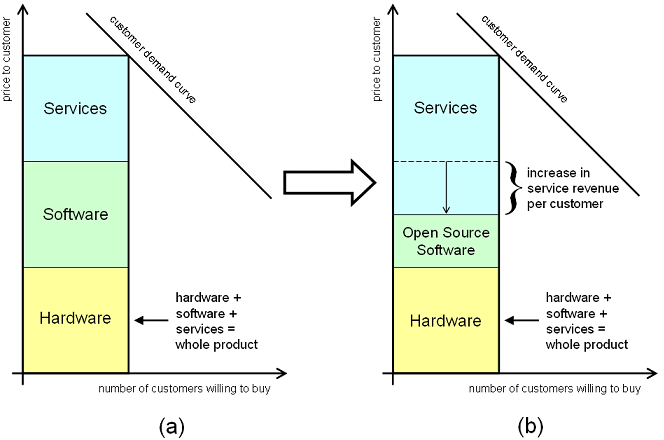
\includegraphics[width=10cm]{figs/it-solutions-demand-curve.png}
    \caption{Taken from The Economic Motivation of Open Source Software: 
Stakeholder Perspectives, by D. Riehle} 
  \end{figure}
\end{center}

\end{frame}

%%%%%%%%%%%%%%%%%%%%%%%%%%%%%%%%%%%%%%%%%%%%%%%%%%%%%%%%%%%%%%%%

\begin{frame}
\frametitle{Business growth in IT markets}

\begin{center}
  \begin{figure}
    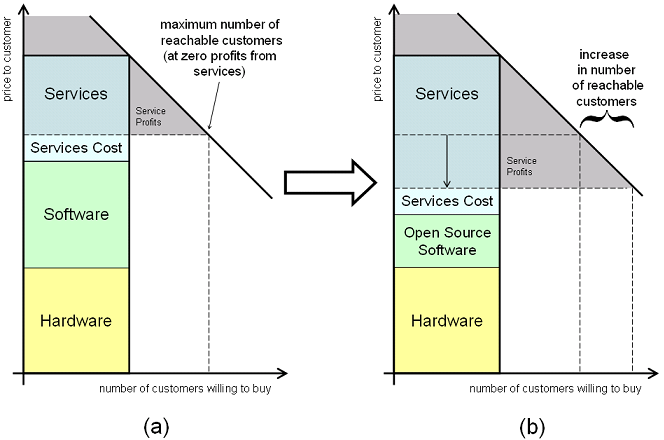
\includegraphics[width=10cm]{figs/business-growth-curve.png}
    \caption{(Taken from The Economic Motivation of Open Source 
Software: Stakeholder Perspectives, by D. Riehle} 
  \end{figure}
\end{center}

\end{frame}

%%%%%%%%%%%%%%%%%%%%%%%%%%%%%%%%%%%%%%%%%%%%%%%%%%%%%%%%%%%%%%%%

\begin{frame}
\frametitle{Single-vendor FLOSS: revenue sources}
\begin{itemize}
  \item Core product.
  \item Whole product.
  \item Operational comfort.
  \item Consulting services.
\end{itemize}
\end{frame}

%%%%%%%%%%%%%%%%%%%%%%%%%%%%%%%%%%%%%%%%%%%%%%%%%%%%%%%%%%%%%%%%

\begin{frame}
\frametitle{Single-vendor also need a community}
\begin{itemize}
  \item FLOSS products without a strong community lead to centralized
development and support problems.
  \item Creating and engaging active communities around single-vendor FLOSS:
  \begin{itemize}
   \item Free use.
   \item No lock-in.
   \item Self support
  \end{itemize}

\end{itemize}
\end{frame}

%%%%%%%%%%%%%%%%%%%%%%%%%%%%%%%%%%%%%%%%%%%%%%%%%%%%%%%%%%%%%%%%

\begin{frame}
\frametitle{Single-vendor: from community to benefits}
\begin{itemize}
  \item Once the single vendor has an active community around its products,
benefits come down the pipe:
  \begin{itemize}
   \item Sales.
   \item Marketing.
   \item Product managment.
   \item Engineering.
   \item Support.
  \end{itemize}

\end{itemize}
\end{frame}

%%%%%%%%%%%%%%%%%%%%%%%%%%%%%%%%%%%%%%%%%%%%%%%%%%%%%%%%%%%%%%%%

\begin{frame}
\frametitle{Example of Single-vendor benefits: sales}
\begin{itemize}
  \item From ``Smoothing the On-ramp to Commercial'', by Larry Augustin.
  \item Single-vendor open source sales funnel (from customers perspective):
  \begin{enumerate}
   \item Download
   \item Install
   \item Use.
   \item Lead.
   \item Prospect
   \item Sale (customer).
  \end{enumerate}

\end{itemize}
\end{frame}

%%%%%%%%%%%%%%%%%%%%%%%%%%%%%%%%%%%%%%%%%%%%%%%%%%%%%%%%%%%%%%%%

\begin{frame}
\frametitle{The role of FLOSS foundations}
\begin{itemize}
  \item Steward of projects under its responsibility.
  \item Financial control, legal coverage and assessment.
  \item Positive added-values: Marketing, public image, negotiations...
  \item The foundation represents the community of developers: 
  \textit{community open source}.
\end{itemize}
\end{frame}

%%%%%%%%%%%%%%%%%%%%%%%%%%%%%%%%%%%%%%%%%%%%%%%%%%%%%%%%%%%%%%%%

\begin{frame}
\frametitle{Market strategy in community FLOSS}

\begin{itemize}
 \item \textit{Law of conservation of attractive profits (Christensen, 2004)}
  \begin{center}
   \begin{quote}
    ``When attractive profits disappear at one stage in the value chain because 
a product becomes modular and commoditized, the opportunity to earn attractive profits 
with proprietary products will usually emerge at an adjacent stage.''
   \end{quote}

  \end{center}

\end{itemize}


\end{frame}

%%%%%%%%%%%%%%%%%%%%%%%%%%%%%%%%%%%%%%%%%%%%%%%%%%%%%%%%%%%%%%%%

\begin{frame}
\frametitle{Market strategy in community FLOSS}
\begin{itemize}
 \item Profits per sale.
\end{itemize}

\begin{center}
  \begin{figure}
    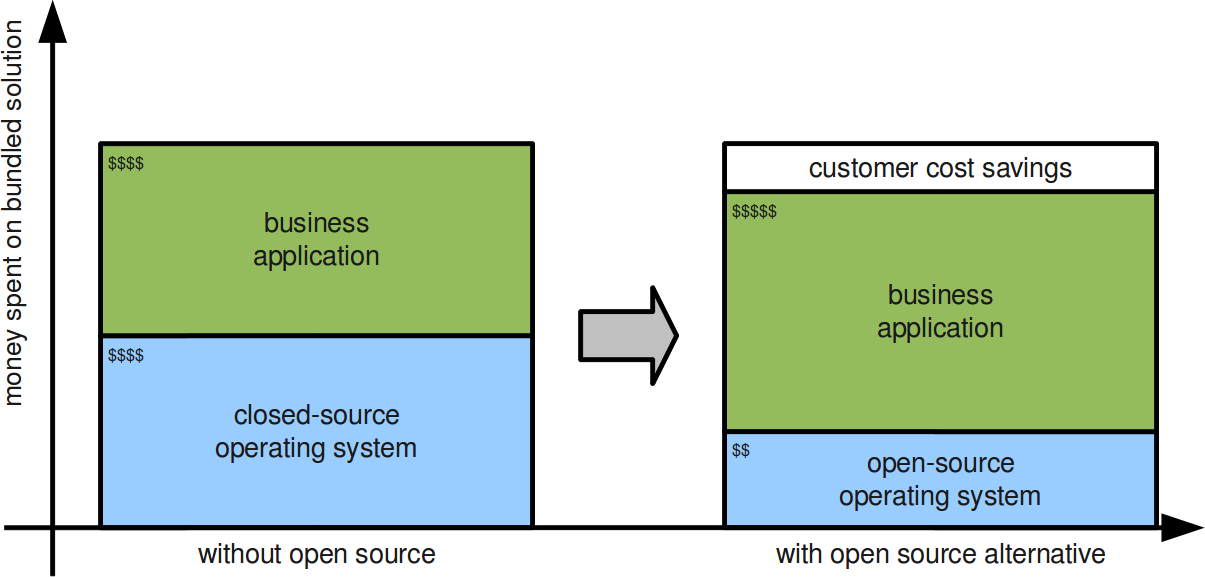
\includegraphics[width=10cm]{figs/floss-vs-closedsw-markets.png}
    \caption{Proprietary software vs. community FLOSS market (from The Economic
Case of Open Source Software Foundations, by D. Riehle)} 
  \end{figure}
\end{center}

\end{frame}

%%%%%%%%%%%%%%%%%%%%%%%%%%%%%%%%%%%%%%%%%%%%%%%%%%%%%%%%%%%%%%%%

\begin{frame}
\frametitle{Market strategy in community FLOSS}

\begin{itemize}
 \item Increased sales in certain market.
\end{itemize}

\begin{center}
  \begin{figure}
    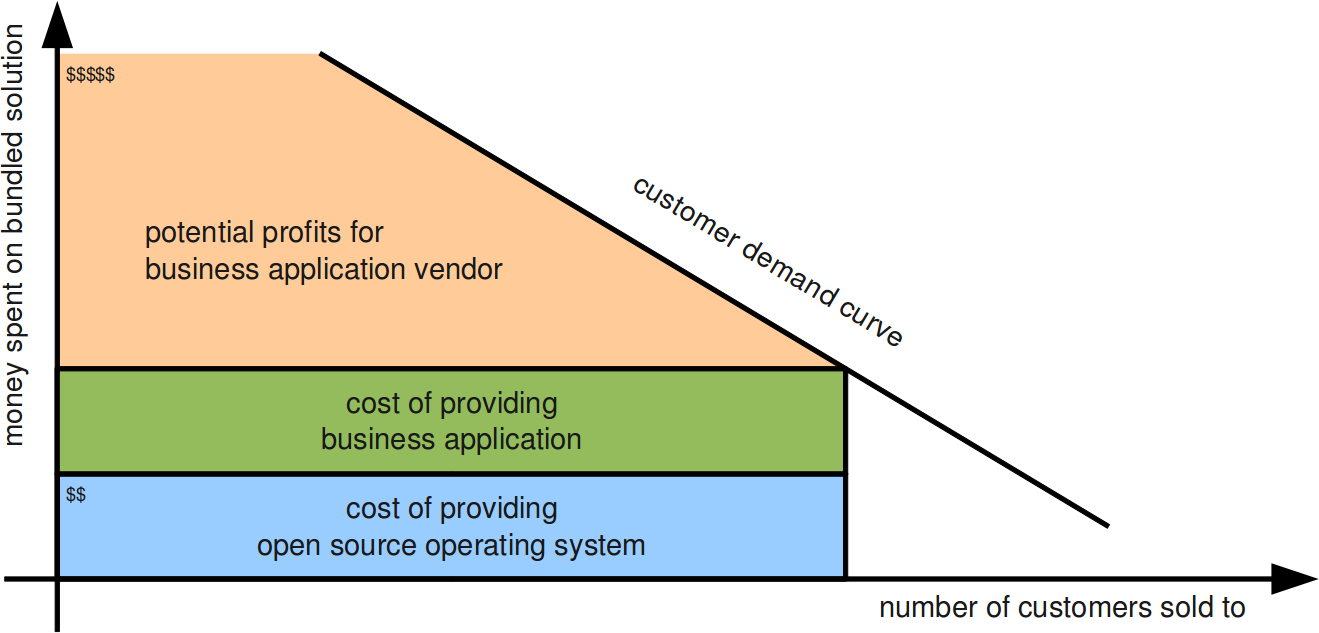
\includegraphics[width=10cm]{figs/customer-demand-curve-floss.png}
    \caption{Customer demand curve in community FLOSS markets (from The Economic
Case of Open Source Software Foundations, by D. Riehle)} 
  \end{figure}
\end{center}

\end{frame}

%%%%%%%%%%%%%%%%%%%%%%%%%%%%%%%%%%%%%%%%%%%%%%%%%%%%%%%%%%%%%%%%

\begin{frame}
\frametitle{Market strategy in community FLOSS}

\begin{itemize}
 \item Larger addressable market.
\end{itemize}

\begin{center}
  \begin{figure}
    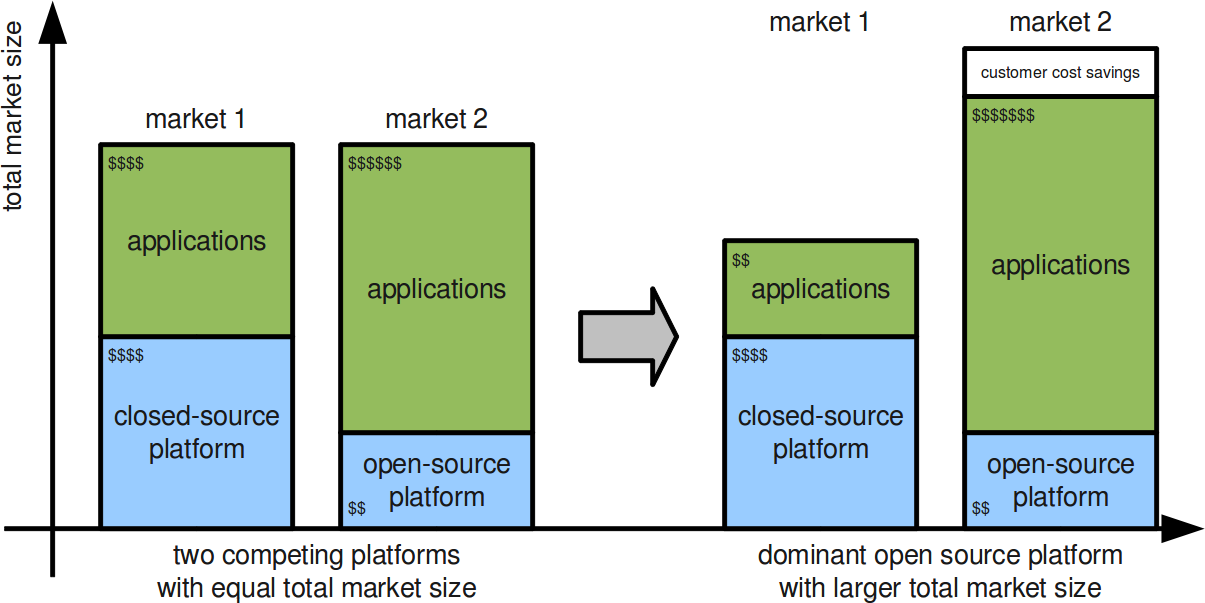
\includegraphics[width=10cm]{figs/growing-floss-platforms-market.png}
    \caption{Larger market size with community FLOSS (from The Economic
Case of Open Source Software Foundations, by D. Riehle)} 
  \end{figure}
\end{center}

\end{frame}

%%%%%%%%%%%%%%%%%%%%%%%%%%%%%%%%%%%%%%%%%%%%%%%%%%%%%%%%%%%%%%%%

\begin{frame}
\frametitle{References}
\begin{itemize}
  \item The Single-Vendor Commercial Open Source Business Model, by D. Riehle.
  \begin{itemize}
   \item \footnotesize{\textit{http://dirkriehle.com/publications/2009/}}
   \footnotetext{\textit{the-commercial-open-source-business-model/}}
  \end{itemize}

  \item The Economic Case for Open Source Foundations, by D. Riehle.
  \begin{itemize}
   \item \footnotesize{\textit{http://dirkriehle.com/publications/2010/}}
   \footnotesize{\textit{the-economic-case-for-open-source-foundations/}}
  \end{itemize}

  \item The Economic Motivation of Open Source Software: Stakeholder Perspectives, by D. Riehle
  \begin{itemize}
   \item \footnotesize{\textit{http://dirkriehle.com/computer-science/research/2007/}}
   \footnotesize{\textit{computer-2007-article.html}}
  \end{itemize}

\end{itemize}
\end{frame}

%%%%%%%%%%%%%%%%%%%%%%%%%%%%%%%%%%%%%%%%%%%%%%%%%%%%%%%%%%%%%%%%

\begin{frame}
\frametitle{References}
\begin{itemize}
  \item The future of open source licensing, by The 451 Group.(Matthew Aslett).
  \begin{itemize}
   \item \footnotesize{\textit{http://blogs.the451group.com/opensource/2010/08/25/}}
    \footnotesize{\textit{the-future-of-open-source-licensing/}}
  \end{itemize}

  \item Estimating savings from OSS code reuse, or: where does the money comes from?, by C. Daffara.
  \begin{itemize}
   \item \footnotesize{\textit{http://carlodaffara.conecta.it/?p=135}}
  \end{itemize}

\end{itemize}
\end{frame}

%%%%%%%%%%%%%%%%%%%%%%%%%%%%%%%%%%%%%%%%%%%%%%%%%%%%%%%%%%%%%%%%
